\documentclass[10pt, a4paper]{article}
\usepackage[utf8]{inputenc}
\usepackage[brazilian]{babel}
\usepackage{lmodern}
\usepackage[left=2cm, right=2cm, top=2cm, bottom=2.5cm]{geometry}
\usepackage{indentfirst}
\usepackage[inline]{enumitem}

\usepackage[pensi]{zeus}

\title{Estudo em Grupo -- Rascunho}
\author{Guilherme Zeus Moura}
\mail{zeusdanmou@gmail.com}
\titlel{Turma Olímpica}
\titler{{\footnotesize v. 1} -- 15 de Abril de 2020}

\begin{document}	
	\zeustitle

	\problem{math/hmmt/2020/A/4}

	\begin{align*}
		\sum_{n=1}^\infty \sum_{k=1}^\infty \frac{\mho(n, k)}{3^{n+k-7}}
		&=\sum_{n=1}^\infty \sum_{k=1}^\infty \frac{3^7}{3^n}\frac{\mho(n, k)}{3^k} \\
		&= 3^7 \cdot \sum_{n=1}^\infty \left( \frac{1}{3^n} \sum_{k=1}^\infty \frac{1}{3^k}\cdot\mho(n, k) \right) \\
		&= 3^7 \cdot \sum_{n=1}^\infty \left( \frac{1}{3^n} \sum_{k=1}^\infty \frac{1}{3^k} \sum_{p | n, p \ge k} 1 \right) \\
		&= 3^7 \cdot \sum_{n=1}^\infty \left( \frac{1}{3^n} \sum_{k=1}^\infty \sum_{p | n, p \ge k}  \frac{1}{3^k} \right) \\
		&= 3^7 \cdot \sum_{n=1}^\infty \left( \frac{1}{3^n}  \sum_{(p, k)\text{ tal que }p | n, p \ge k} \frac{1}{3^k} \right) \\
		&= 3^7 \cdot \sum_{n=1}^\infty \left( \frac{1}{3^n}  \sum_{p | n} \sum_{1 \le k\le p} \frac{1}{3^k} \right) \\
		&= 3^7 \cdot \sum_{n=1}^\infty \left( \frac{1}{3^n}  \sum_{p | n} \left( \frac{1}{3} + \frac{1}{3^2} \cdots + \frac{1}{3^p} \right)\right) \\
		&= 3^7 \cdot \sum_{n=1}^\infty \left( \frac{1}{3^n}  \sum_{p | n} \frac{1 - \frac{1}{3^p}}{2}\right)
	\end{align*}
	\begin{align*}
		\sum_{n=1}^\infty \sum_{k=1}^\infty \frac{\mho(n, k)}{3^{n+k-7}}
		&= \frac{3^7}{2} \cdot \sum_{n=1}^\infty \left( \frac{1}{3^n}  \sum_{p | n} \left(1 - \frac{1}{3^p}\right) \right) \\
		&= \frac{3^7}{2} \cdot \sum_{n=1}^\infty \sum_{p|n} \left( \frac{1}{3^n}  \left(1 - \frac{1}{3^p}\right) \right) \\
		&= \frac{3^7}{2} \cdot \sum_{p\text{ primo}} \sum_{n = tp} \left( \frac{1}{3^n}  \left(1 - \frac{1}{3^p}\right) \right) \\	
		&= \frac{3^7}{2} \cdot \sum_{p\text{ primo}} \sum_{t = 1}^\infty \left( \frac{1}{3^{tp}}  \left(1 - \frac{1}{3^p}\right) \right) \\	
		&= \frac{3^7}{2} \cdot \sum_{p\text{ primo}} \left( \left( 1 - \frac{1}{3^p} \right) \sum_{t = 1}^\infty \left(\frac{1}{3^{p}}\right)^t \right) \\	
		&= \frac{3^7}{2} \cdot \sum_{p\text{ primo}} \left( \left( 1 - \frac{1}{3^p} \right) \sum_{t = 1}^\infty \left(\frac{1}{3^{p}}\right)^t \right) \\	
		&= \frac{3^7}{2} \cdot \sum_{p\text{ primo}} \left( \left( \frac{3^p - 1}{3^p} \right) \left(\frac{1}{3^{p} - 1}\right) \right) \\	
		&= \frac{3^7}{2} \cdot \sum_{p\text{ primo}} \left( \frac{1}{3^p} \right) \\	
		&= \frac{3^7}{2} \cdot \left( \frac{1}{3^2} + \frac{1}{3^3} + \frac{1}{3^5} + \frac{1}{3^7} + \frac{1}{3^{11}} + \frac{1}{3^{13}} + \cdots \right) \\
	\end{align*}

	\newpage
	\problem{math/imosl/2009/C1}

	\begin{idea}
		Considere uma sequência de algarismos 0's e 1's, em base binária, correspondendo cartas de ouro com o algarismo 1 e cartas pretas com o algarismo 0. Observe que esse novo ``número'', resultado da concatenação dos algarismos, sempre diminui -- é monovariante.
	\end{idea}


	\begin{idea}
		Vamos chamar de \emph{cartas quinquagésimas} as cartas tal que o número de cartas entre (inclusivo) ela e a carta mais a direita é um múltiplo de 50. A paridade do número de cartas quinquagésimas com face ouro sempre muda a cada movimento.
	\end{idea}

	\newpage \setcounter{prob}{3}
	\begin{prob}
		A maze consists of a finite grid of squares where the boundary and some internal
edges are “walls” that cannot be crossed. For example:

	\begin{center}
		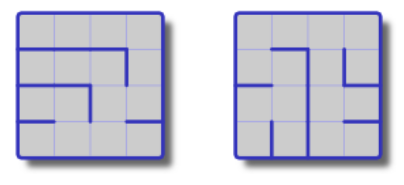
\includegraphics[width=0.4\textwidth]{pic.png}
	\end{center}

	Two mazes are given, each with a robot in the top-left square. You may give a list of directions
(up, down, left, or right) to the robots. Both robots will independently follow the same list of directions. For each direction, the robot will move one square in that direction if it can, or do
nothing if there is a wall in the way. It will then proceed to the next direction, and repeat until it
has gone through the whole list. Suppose that there is a list of directions that will get each robot
individually from the top-left corner to the bottom-right corner of its maze. Prove there is also a
list of directions that will get both robots to the bottom-right corner at the same time.

In the example mazes above, you could give the directions ‘Right’, ‘Right’, ‘Down’, ‘Down’,
‘Down’, ‘Right’, ‘Down’, ‘Down’, ‘Left’, ‘Down’, ‘Right’.
	\end{prob}

	\begin{idea}
		Levar o primeiro robô até o objetivo. Levar o segundo robô até o objetivo e ver o que acontece com a distância do primeiro robô até o objetivo.
	\end{idea}

\end{document}
